\section{ТРИГОНОМЕТРИЯ}

\textbf{2222.}

{\centering 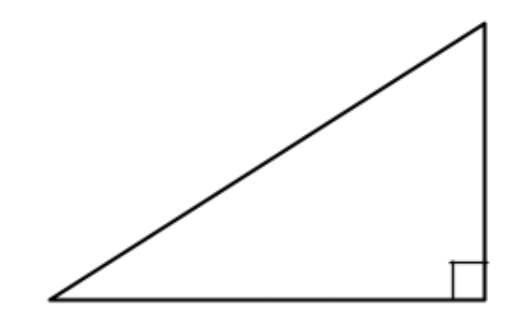
\includegraphics[width=0.35\linewidth]{Geometry/Content/51.png}
	
}

В прямоугольном треугольнике принято вершины (и соответствующие углы) обозначать прописными (заглавными) буквами: $A$, $B$, $C$. Прямой угол обычно обозначают буквой $C$. Стороны треугольника, противолежащие углам, обычно обозначают теми же буквами, но строчными (малыми): $a$, $b$, $c$.

Синусом острого угла называется отношение противолежащего катета к гипотенузе:
\[
\sin{A} = \frac{a}{c}, \;\; \sin{B}=\frac{b}{c}.
\]
Косинусом острого угла называется отношение прилежащего катета к гипотенузе:
\[
\cos{A} = \frac{b}{c}, \;\; \cos{B}=\frac{a}{c}.
\]
Очевидно, в прямоугольном треугольнике:
\[
\sin{A} = \cos{B}, \;\; \cos{A} = \sin{B}.
\]
Синус угла через его косинус и наоборот вычисляются по формулам:
\[
\sin{A} = \sqrt{1-\cos^2{A}}, \;\; \cos{A} = \sqrt{1 - \sin^2{A}}.
\]
 Эти соотношения (и другие, которые приведем в свое время) широко используются для простейших вычислений в прямоугольном треугольнике.
 
 В нашем случае  $\sin{A} = \frac{\sqrt{15}}{4}$, следовательно $\cos{A}=\sqrt{1 - \frac{15}{16}}=\frac{1}{4}.$ 
 
 \null \hspace*{\fill} Ответ: 0,25.
 
 \textbf{2223-2226} $-$ аналогичные задачи.
 
 \textbf{2227.} $\sin{B} = \cos{A} = \sqrt{1-\sin^{A}}=\sqrt{1-\frac{7}{16}}=\frac{3}{4}$ \newline \null \hspace*{\fill} Ответ: 0,75.
 
 \textbf{2228,2229} $-$ аналогичные задачи
 
 \textbf{2230.} Тангенсом угла в прямоугольном треугольнике называется отношение противолежащего и прилежащего катетов. Он равен отношению синуса и косинуса данного угла:
 \[
 tg\;A = \frac{\sin{A}}{\cos{A}} = \frac{a}{b}.
 \]
 Если известно значение $\cos{A}$, то $1+tg^2A=\frac{1}{\cos^2{A}}$ и тангенс можно вычислить по формуле:
 \[
 tg\;A=\sqrt{\frac{1}{\cos^2{A}} - 1}.
 \]
 В данной задаче $tg\;A=\sqrt{\frac{1}{\cos^2{A}} - 1} = \sqrt{\frac{89}{25} - 1} = \frac{8}{5}=1,6$. \newline \null \hspace*{\fill} Ответ: 1,6.
 
 \textbf{2231,2232} $-$ аналогичные задачи.
 
 \textbf{2233.} $tg\;A=\frac{\sin{A}}{\cos{A}}=\frac{\sin{A}}{\sqrt{1-\sin^{A}}} = \frac{9/\sqrt{181}}{\sqrt{1 - 81/181}}=\frac{9}{10}=0,9.$ \newline \null \hspace*{\fill} Ответ: 0,9.
 
 \textbf{2234.} $1 + tg^2A=\frac{1}{\cos^2{A}}$, $\cos{A} = \frac{1}{\sqrt{1+tg^2A}}=\frac{1}{\sqrt{1+24}} = 0,2.$ \newline \null \hspace*{\fill} Ответ: 0,2.
 
 \textbf{2235} $-$ аналогичная задача.
 
 \textbf{2236.} $\sin{A} = tg\; A\cdot \cos{A} = \frac{tg\;A}{\sqrt{1+tg^2A}}=\frac{1/\sqrt{3}}{\sqrt{1+1/3}}=\frac{1}{2}=0,5$. \newline \null \hspace*{\fill} Ответ: 0,5.
 
 \textbf{2237-2241} $-$ решаются аналогично.
 
 \clearpage
 \textbf{2242.}
 
 {\centering 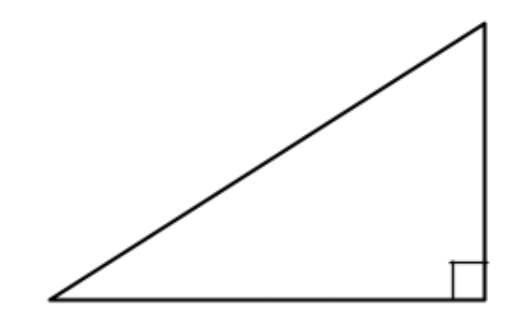
\includegraphics[width=0.4\linewidth]{Geometry/Content/51.png}
 	
 }
\[
BC=AB\sin{A}=10\cdot0,9=9.
\]
\null \hspace*{\fill} Ответ: 9.

\textbf{2243-2245} $-$ решаются аналогично, т.е. через тригонометрические функции острых углов прямоугольного треугольника.

\textbf{2246.} (см. чертеж задачи \textbf{2242}). $\cos{A} = \sqrt{1-\left( \frac{\sqrt{21}}{5} \right)^2} = \frac{5}{2}.$ $AC=AB\cos{A}=10\cdot\frac{2}{5}=4.$ \newline \null \hspace*{\fill} Ответ: 4.

\textbf{2247-2249} $-$ аналогичные задачи.

\textbf{2250.} (см. чертеж задачи \textbf{2242}). $\cos{A} = \sqrt{1-\sin^2{A}} = \linebreak= \sqrt{1-0,01}=\sqrt{\frac{99}{100}}=\frac{3\sqrt{11}}{10}$. Тогда $AB=\frac{AC}{\cos{A}}=\frac{3\sqrt{11}}{3\sqrt{11}/10}=10.$ \newline \null \hspace*{\fill} Ответ: 10.

\textbf{2251-2253} $-$ аналогичные задачи.

\textbf{2254.} 
 
{\centering 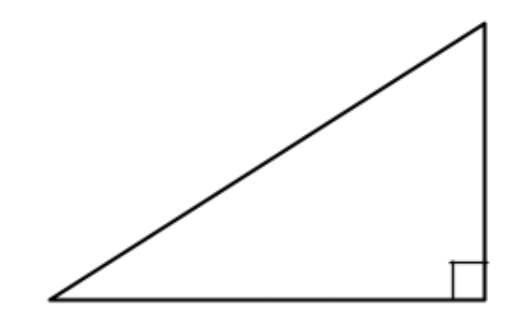
\includegraphics[width=0.4\linewidth]{Geometry/Content/51.png}
	
}
\[
BC = AC\cdot tg\;A =20\cdot 0,2=4.
\] \null \hspace*{\fill} Ответ: 4.

\textbf{2255-2257} $-$ аналогичные задачи.

\textbf{2258.} (см. чертеж задачи \textbf{2254}). $\cos{A}=\frac{1}{\sqrt{1+tg^2A}}=\frac{1}{\sqrt{1 + \left( \frac{7}{24} \right)^2}} = \linebreak= \frac{24}{25}$,  
так что $AC=AB\cdot\cos{A}=\frac{5\cdot24}{25}=4,8.$ \newline \null \hspace*{\fill} Ответ: 4,8.

\textbf{2259-2261} $-$ аналогичные задачи.

\textbf{2262.}

{\centering 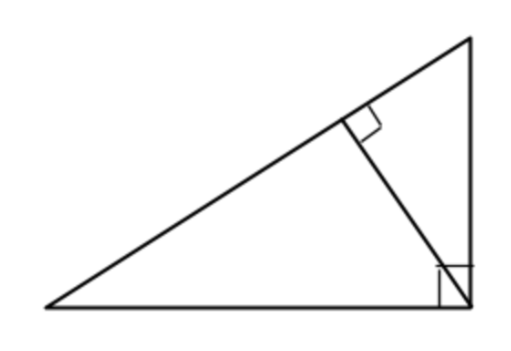
\includegraphics[width=0.4\linewidth]{Geometry/Content/52.png}
	
}

Из треугольника $ABC$ $BC=AB\cdot\sin{A}=16\cdot\frac{3}{4}=12$.

Из прямоугольного треугольника $HBC$ $BH=BC\cdot\cos{B}=\linebreak=BC\cdot\sin{A}=12\cdot\frac{3}{4}=9.$ \newline \null \hspace*{\fill} Ответ: 9.

Практически все задачи \textbf{2263-2281} решаются с помощью чертежа к задаче \textbf{2254} (все три треугольника: $ABC$, $HBC$ и $HAC$ $-$ являются прямоугольными, с одинаковыми парами острых углов). Можно для решения таких задач использовать и тот факт, что они подобные. 

\textbf{2282.}

{\centering 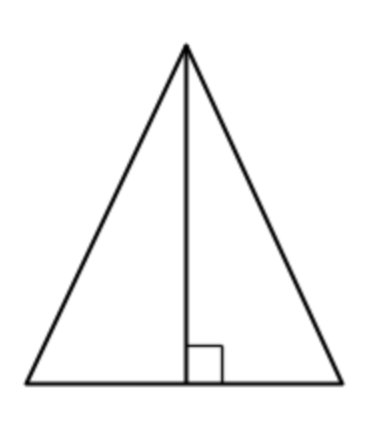
\includegraphics[width=0.35\linewidth]{Geometry/Content/53.png}
	
}

Т.к. $AC=BC$,  треугольник $ABC$ $-$ равнобедренный. Проведем высоту $CH \perp AB$, которая является и медианой. Тогда $AH=\linebreak=BH=\frac{AB}{2}=4$. Теперь из прямоугольного треугольника $CAH$:
\[
AC=\frac{AH}{\cos{A}}=\frac{4}{0,2}=20.
\] \null \hspace*{\fill} Ответ: 20.

 Задачи \textbf{2283-2289} решаются аналогично на основании чертежа задачи \textbf{2282}.
 
 \textbf{2290.} См. чертеж задачи \textbf{2282}. Т.к. $CH \perp AB$, треугольник $CAH$ - прямоугольный. Тогда
 \[
 AH=AC\cos{A} =\frac{AC}{\sqrt{1+tg^2A}}=\frac{15}{\sqrt{1+ \left( \frac{4}{3} \right)^2}}=15\cdot\frac{3}{5}=9
 \] 
 треугольник $ABC$ $-$ равнобедренный, то $AB=2AH=18$. \newline \null \hspace*{\fill} Ответ: 18.
 
 \textbf{2291-2303} $-$ легко решаются с использованием все того же чертежа и соотношений между тригонометрическими функциями прямоугольного треугольника.
 
 \textbf{2304.} Проведем высоту $BH\perp AC$. Из прямоугольного треугольника $ABH$:
 \[
 BH = AB\sin{A}=AB\cdot\sqrt{1-\cos^2{A}}=21\cdot\sqrt{1-\frac{40}{49}}=21\cdot\frac{3}{7}=9.
 \] \null \hspace*{\fill} Ответ: 9.
 
 \textbf{2305} $-$ аналогичная задача.
 
 \textbf{2306.}
 
 Треугольник $ABC$ $-$ равнобедренный, высота $CH \perp AB$ является медианой, $AH=BH=\frac{AB}{2}=25$. Из прямоугольного треугольника $CAH$:
 \begin{multline*}
 CH=AH\;tg\;A=\frac{AH\cdot\sin{A}}{\cos{A}}=\frac{Ah\cdot\sin{A}}{\sqrt{1-\sin^2{A}}}=\\=\frac{25\cdot \frac{12}{13}}{\sqrt{1-\frac{144}{169}}} =\frac{25\cdot\frac{12}{12}}{\frac{5}{13}} = 60.
 \end{multline*} \null \hspace*{\fill} Ответ: 60.

Все остальные задачи данного раздела решаются аналогично.